\subsection{Poles, zeros and RGA}

The system is modelized as a MIMO system with two inputs ($u_1 \& u_2$) and two ouputs ($y_1 \& y_2$).
The multivariable model with $2$ inputs and $2$ outputs is given by $Y(s) = G(s)U(s)$.
Depending on the settings of the valves -- minimum/maximum phase model -- we obtain different $G(s)$.
Each exercise in the following take care of the two settings.

\subsubsection{Exercise}
\paragraph{Minimum phase model}

The transfer matrix $G_{mp}(s)$ is:

$$G_{mp}(s) = \left(\begin{array}{cc} 
    \frac{.035}{s + .056} & \frac{.00046}{s^2 + .082 s + .0015} \\
    \\
    \frac{ .00044}{  s^2 + .073 s + .0011} & \frac{.030}{s + .052} \\
\end{array}\right)$$


Poles and zeros of the elements are given in the following table:

$$
\text{Poles}(G_{mp,i,j}(s)) = \left(\begin{array}{cc} -.056 & \left(\begin{array}{c} -.056\\ -.026 \end{array}\right) \\ \left(\begin{array}{c} -.052\\ -.021 \end{array}\right) & -.052 \\ \end{array}\right)
$$

$$\text{Zeros}(G_{mp,i,j}(s)) = \emptyset $$

\paragraph{Non-minimum phase model}

The transfer matrix $G_{nmp}(s)$ is:

$$G_{nmp}(s) = \left(\begin{array}{cc} 
    \frac{.021}{s + .051} & \frac{.0026}{s^2 + .14 s + .0044} \\
    \\
    \frac{ .0032}{ s^2 + .14 s + .0043} & \frac{.018}{s + .047} \\
\end{array}\right)$$

Poles and zeros of the elements are given in the following table:


$$\text{Poles}(G_{nmp,i,j}(s)) = 
\left(\begin{array}{cc} -.051 & \left(\begin{array}{c} -.086\\ -.051 \end{array}\right) \\ \left(\begin{array}{c} -.091\\ -.047 \end{array}\right) & -.047 \\ \end{array}\right)
$$

$$\text{Zeros}(G_{nmp,i,j}(s)) = \emptyset $$

\subsubsection{Exercice}

\paragraph{Minimum phase model}

Poles and zeros of the multivariable system in the minimum phase model case are:

$$\begin{array}{rcl}
    \text{Poles} & = & 
    \left(\begin{array}{c}  
            -.056 \text{ (double)} \\
            -.052 \text{ (double)} \\
    -.021 \\
    -.026 \\
    \end{array}\right) \\ 
    \text{Zeros} & = & 
    \left(\begin{array}{c}
              -.0093 \\
                 -.038 \\
                    -.056 \\
                       -.052 \\
    \end{array}\right)
\end{array}
    $$

\paragraph{Non-minimum phase model}

Poles and zeros of the multivariable system in the minimum phase model case are:

$$
Prout
$$


% \subsubsection{Exercise}
\lipsum[1-1]

% \subsubsection{Exercice}
\paragraph{Minimum phase model}

The RGA of the minimum phase system at frequency $0$ is:

\begin{multline*} 
    \text{RGA}(G_{mp}(0)) = \\
    G_{mp}(0) .* [G_{mp}^{-1}(0)]^T = \\
    \left(\begin{array}{cc} 1.6 & -0.56\\ -0.56 & 1.6 \end{array}\right)
\end{multline*}

Using the second rule of thumb expressed in the subject gives the following result:

\begin{center}
\begin{tabular}{|c|cc|}
    \hline
    \backslashbox{Out}{In}& 1 & 2 \\
    \hline
        1 & $1$ & $0$ \\
        2 & $0$ & $1$ \\
    \hline
\end{tabular} \ \\ \ \\
($0$ -- avoid pairing, $1$ -- pairing possible).
\end{center}

\paragraph{Non-minimum phase model}

The RGA of the non-minimum phase system at frequency $0$ is:

\begin{multline*}
    \text{RGA}(G_{nmp}(0)) = \\ 
    G_{nmp}(0) .* [G_{nmp}^{-1}(0)]^T =  \\
    \left(\begin{array}{cc} -0.56 & 1.6\\ 1.6 & -0.56 \end{array}\right)
\end{multline*}

Using the second rule of thumb expressed in the subject gives the following result:

\begin{center}
\begin{tabular}{|c|cc|}
    \hline
    \backslashbox{Out}{In}& 1 & 2 \\
    \hline
        1 & $0$ & $1$ \\
        2 & $1$ & $0$ \\
    \hline
\end{tabular} \ \\ \ \\
($0$ -- avoid pairing, $1$ -- pairing possible).
\end{center}


\textbf{Remark:} The two RGA matrix at frequency $0$ are symetrical. This seems legit since the alimentation of tanks 1 \& 4 is made by pump 1 and the alimentation of tanks 2 \& 3 is made by pump 2.

% \subsubsection{Exercise}
\lipsum[1-1]

% \subsubsection{Exercise}

The impact of each input can be measured as: $$\frac{|y_{\text{paired to } u_i}|}{|y_{\text{not-paired}}|}$$

We have the following relation:
\begin{shortitemize}
    \item Input (1):
$$\frac{|y_{1,m}|_\infty}{|y_{2,m}|_\infty} = \frac{.6}{.4} = 1.5 \leq \frac{|y_{2,nm}|_\infty}{|y_{1,nm}|_\infty} = \frac{.7}{.4} = 1.75$$  
    \item Input (2):
$$\frac{|y_{2,m}|_\infty}{|y_{1,m}|_\infty} = \frac{.6}{.3} = 2 \geq \frac{|y_{1,nm}|_\infty}{|y_{2,nm}|_\infty} = \frac{.6}{.4} = 1.5$$ 
\end{shortitemize}

This result can be sum up as:

\begin{center}
\begin{tabular}{|c|cc|}
    \hline
    Desired control & $y_1$ & $y_2$ \\ 
    \hline
    \multirow{2}*{$G_m(s)$} & Act on $u_1$ & Act on $u_2$ \\ 
                & \emph{Stronger} & \emph{Weaker}\\
                & \emph{coupling} & \emph{coupling} \\ 
    \hline
    \multirow{2}*{$G_{nm}(s)$} & Act on $u_2$ & Act on $u_1$ \\
             & \emph{Weaker} & \emph{Stronger}\\
             & \emph{coupling} & \emph{coupling} \\
    \hline
\end{tabular}
\end{center}

\begin{figure}[h!t]
    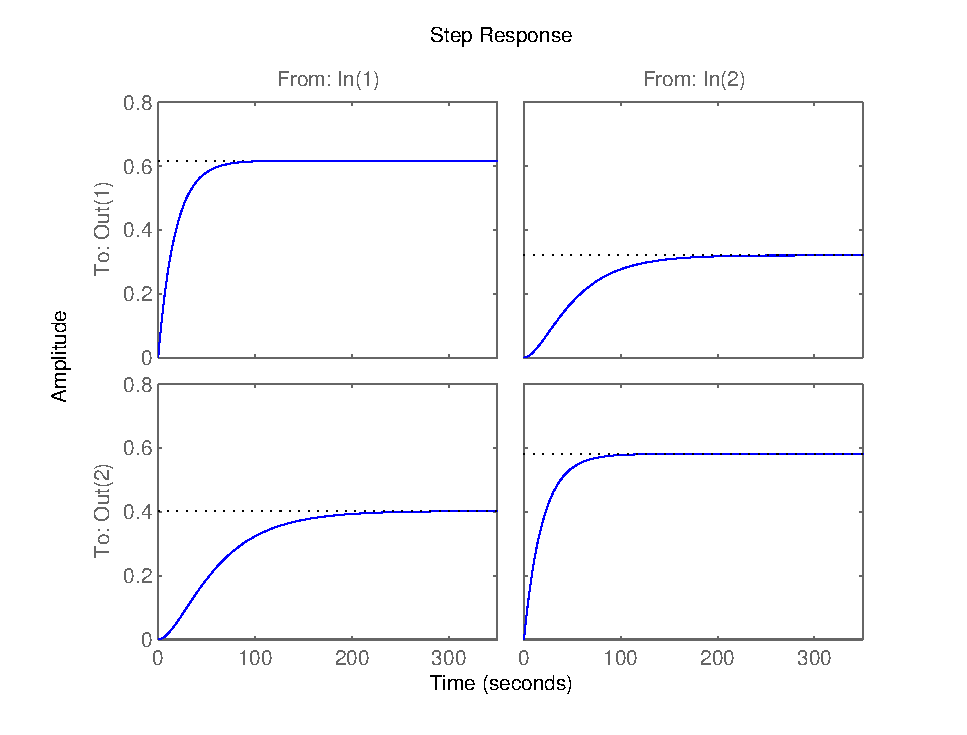
\includegraphics[width=\columnwidth]{fig/step315m}
    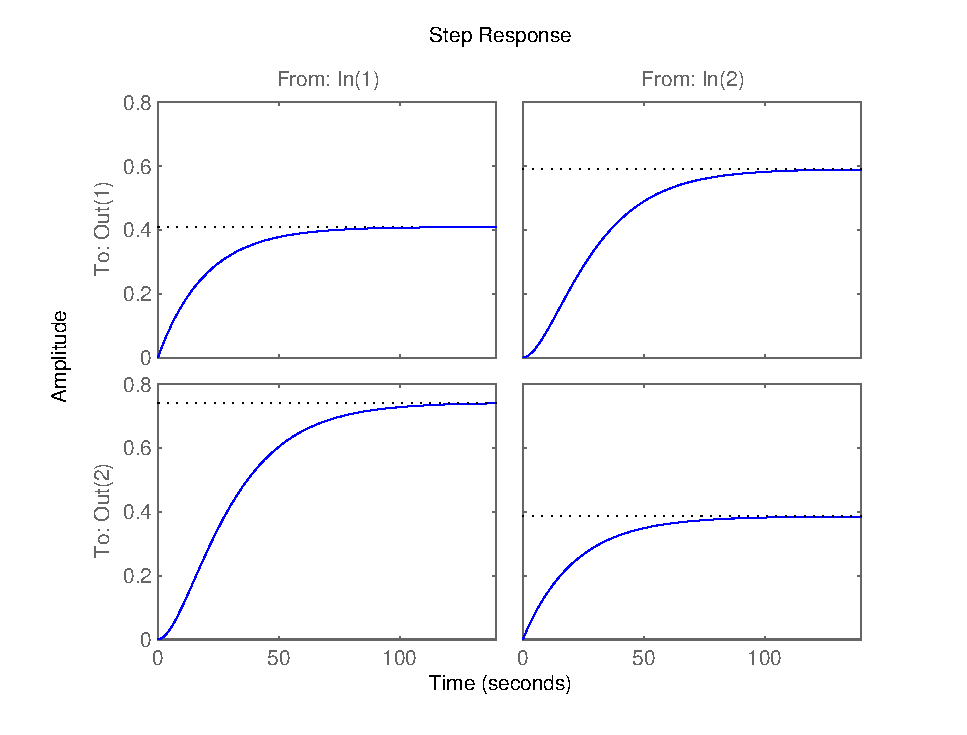
\includegraphics[width=\columnwidth]{fig/step315nm}
    \caption{Step responses of the systems \\ Minimum phase system (top) and non-minimum phase system (bottom)}    
    \label{step315}
\end{figure}

